
\documentclass[11pt,a4paper]{article}
\usepackage{fontspec}
\defaultfontfeatures{Ligatures=TeX}
\IfFontExistsTF{Times New Roman}{\setmainfont{Times New Roman}}{\setmainfont{TeX Gyre Termes}}

\usepackage{geometry}
\geometry{a4paper, left=15mm, right=15mm, top=12mm, bottom=15mm}
\usepackage{tabularx}
\usepackage{amssymb}
\usepackage{xcolor}
\usepackage{colortbl}
\usepackage{ifthen}
\usepackage{graphicx}
\usepackage{array}
\usepackage{tcolorbox}
\usepackage{tikz}

\setlength{\parindent}{0pt}
\setlength{\parskip}{0.22em}

\newcolumntype{Y}{>{\centering\arraybackslash}X}

% Custom Checkbox macro
\newcommand{\CheckBox}[2][false]{%
    \ifthenelse{\equal{#1}{true}}{%
        \makebox[0pt][l]{$\square$}\raisebox{.15ex}{\hspace{0.08em}$\checkmark$}%
    }{%
        $\square$%
    }%
    \hspace{0.12cm}#2%
}

% Section & Subsection Headers
\newcommand{\SectionTitle}[2]{%
    \vspace{0.12cm}
    {\bfseries\large #1/ \textit{#2}}\par
    \vspace{0.06cm}
}

\newcommand{\SubSectionTitle}[2]{%
    \vspace{0.08cm}
    {\bfseries #1/ \textit{#2}}\par
}

% Page Footer
\newcommand{\FormFooter}[2]{%
    \vfill
    \hrule
    \vspace{0.08cm}
    \noindent
    \small \textcolor{gray}{VM - BS - V1 - 012} \hfill \small \textcolor{gray}{Trang #1 / Page #2}
}

% VAS Pain Scale Components
\newcommand{\VASGuidanceBox}{%
    \noindent
    \begin{tcolorbox}[colback=white,colframe=gray!70,arc=0mm,boxrule=0.5pt,top=2mm,bottom=2mm,left=3mm,right=3mm]
        \small
        Chúng tôi khuyên bạn nên sử dụng thang điểm để giúp bạn đo mức độ đau\\
        \textit{We advise you to use a pain thermometer to help you measure the intensity of the pain:}\\[0.1cm]
        Cường độ đau có thể xác định bằng đường thẳng như ví dụ dưới đây\\
        \textit{Pain intensity can be defined with a line like the one in the example below:}\\[0.1cm]
        Một đầu thể hiện <<mức đau cao nhất có thể>>, điểm đau càng lệch về đầu này cơn đau càng nhiều\\
        \textit{One extremity shows the <<maximum imaginable pain>>, more the line is near to the end, your pain is worse.}\\[0.1cm]
        Một đầu khác thể hiện mức <<không đau>>, nếu điểm đau càng lệch về đầu này cơn đau càng ít\\
        \textit{The other extremity shows that there is <<no pain>>, if the line is near to the start, it means you do not feel any pain.}\\[0.15cm]
        \begin{tabularx}{\textwidth}{@{} l X r @{}}
            \small Không đau & \rule[0.5ex]{\linewidth}{0.6pt} & \small Mức đau cao nhất có thể \\
            \small\textit{No pain} & & \small\textit{Maximum imaginable pain} \\
        \end{tabularx}
    \end{tcolorbox}
}

\newcommand{\VASScaleCell}[2]{%
    \ifthenelse{\equal{#1}{#2}}{%
        \tikz[baseline=(char.base)]{\node[shape=circle,draw=black,thick,inner sep=1.2pt] (char) {\textbf{#2}};}%
    }{%
        #2%
    }%
}

\newcommand{\VASScaleBar}[3]{%
    \vspace{0.15cm}
    \noindent\textbf{#1}\par
    \noindent\textit{#2}\\[0.08cm]
    \noindent
    \begin{tabularx}{\textwidth}{|*{11}{Y|}}
        \hline
        \rowcolor{gray!15}
        \VASScaleCell{#3}{0} & 
        \VASScaleCell{#3}{1} & 
        \VASScaleCell{#3}{2} & 
        \VASScaleCell{#3}{3} & 
        \VASScaleCell{#3}{4} & 
        \VASScaleCell{#3}{5} & 
        \VASScaleCell{#3}{6} & 
        \VASScaleCell{#3}{7} & 
        \VASScaleCell{#3}{8} & 
        \VASScaleCell{#3}{9} & 
        \VASScaleCell{#3}{10} \\
        \hline
    \end{tabularx}\\[0.05cm]
    \noindent{\small Không đau/ \textit{None}} \hfill {\small Đau nhiều nhất/ \textit{Max}}\par
}

% 6-Column Horizontal Rating Scale Row
\newcommand{\HorizontalRatingRow}[4]{%
    % #1: Question VI, #2: Question EN, #3: Selected col (1..6 or empty), #4: Note
    \vspace{0.1cm}
    \noindent\textbf{#1}\par
    \noindent\textit{#2} \ifx&#4&\else\hspace{0.5cm}\underline{~#4~}\fi\\[0.05cm]
    \noindent
    \begin{tabularx}{\textwidth}{|*{6}{Y|}}
        \hline
        \rowcolor{gray!10}
        \small Không bao giờ & \small Không rõ & \small Ít khi & \small Thường xuyên & \small Nhiều & \small Rất nhiều \\
        \textit{\footnotesize Never} & \textit{\footnotesize Hardly noticed} & \textit{\footnotesize Slightly} & \textit{\footnotesize Moderately} & \textit{\footnotesize Strongly} & \textit{\footnotesize Very strongly} \\
        \hline
        \ifthenelse{\equal{#3}{1}}{\makebox[0pt][l]{$\square$}\raisebox{.15ex}{\hspace{0.08em}$\checkmark$}}{$\square$} & 
        \ifthenelse{\equal{#3}{2}}{\makebox[0pt][l]{$\square$}\raisebox{.15ex}{\hspace{0.08em}$\checkmark$}}{$\square$} & 
        \ifthenelse{\equal{#3}{3}}{\makebox[0pt][l]{$\square$}\raisebox{.15ex}{\hspace{0.08em}$\checkmark$}}{$\square$} & 
        \ifthenelse{\equal{#3}{4}}{\makebox[0pt][l]{$\square$}\raisebox{.15ex}{\hspace{0.08em}$\checkmark$}}{$\square$} & 
        \ifthenelse{\equal{#3}{5}}{\makebox[0pt][l]{$\square$}\raisebox{.15ex}{\hspace{0.08em}$\checkmark$}}{$\square$} & 
        \ifthenelse{\equal{#3}{6}}{\makebox[0pt][l]{$\square$}\raisebox{.15ex}{\hspace{0.08em}$\checkmark$}}{$\square$} \\
        \hline
    \end{tabularx}
}

% Numbered Option for Questionnaire (BDI Style)
\newcommand{\NumberedOption}[4][false]{%
    \hspace*{0.3cm}#2 \hspace{0.15cm}\CheckBox[#1]{#3/ \textit{#4}}\par\vspace{0.04cm}
}

% Follow-up Block Macro
\newcommand{\FollowUpBlock}{%
    \noindent\textbf{Ngày/ \textit{Date}:} \dotfill\\[0.12cm]
    \noindent\textbf{Bác sỹ điều trị/ \textit{Physician}:} \dotfill\\[0.12cm]
    \noindent\textbf{Bước tiếp theo/ \textit{Next step}:} \dotfill\\[0.12cm]
    \noindent\textbf{Lần khám tiếp theo/ \textit{Next appointment}:} \dotfill\par
    \vspace{0.08cm}
    \hrule
    \vspace{0.12cm}
}

\begin{document}


\noindent
\begin{minipage}{0.5\textwidth}
    \includegraphics[height=1.2cm,keepaspectratio]{ images/logo.jpg }
\end{minipage}

\vspace{0.3cm}
\begin{center}
    {\bfseries\LARGE BỆNH ÁN ĐAU TOÀN DIỆN}\\[0.1cm]
    {\bfseries\large COMPREHENSIVE PAIN RECORD}
\end{center}
\vspace{0.25cm}

\textbf{ Bác sỹ điều trị đau/ \textit{ Pain Clinic Physician }: } \underline{~Bác sĩ Vũ Hữu Nam~}\\[0.12cm]
\textbf{ Người bệnh/ \textit{ Patient }: } \underline{~Đặng Quốc Lâm~}\\[0.12cm]
\textbf{ Mã người bệnh/ \textit{ PID }: } \underline{~VM2026-0152~}\\[0.12cm]
\textbf{ Hội chứng chính/ \textit{ Main syndrome }: } \underline{~Viêm quanh khớp vai / rách gân chóp xoay~}\\[0.12cm]
\textbf{ Ngày khám đầu/ \textit{ Date of first Visit }: } \underline{~30/09/2026~} ~~~~~ \textbf{ Điều dưỡng/ \textit{ Nurse }: } \underline{~N/A~}\\[0.12cm]
\vspace{0.15cm}
\hrule
\vspace{0.15cm}

\SectionTitle{ THÔNG TIN NGƯỜI BỆNH }{ PATIENT INFORMATION }

\textbf{ Ngày sinh/ \textit{ Date of Birth }: } \underline{~N/A~} ~~~~~ \textbf{ Tuổi/ \textit{ Age }: } \underline{~52~} ~~~~~ \textbf{ Giới tính/ \textit{ Gender }: } \underline{~Nam~}\\[0.12cm]
\textbf{ Địa chỉ/ \textit{ Address }: } \underline{~Xã Tiền Phong, Mê Linh, Hà Nội~}\\[0.12cm]
\textbf{ Đất nước/ \textit{ Country }: } \underline{~Việt Nam~} ~~~~~ \textbf{ Quốc tịch/ \textit{ Nationality }: } \underline{~Việt Nam~}\\[0.12cm]
\textbf{ Email/ \textit{ Email }: } \underline{~N/A~} ~~~~~ \textbf{ ĐT nhà/ \textit{ Home No }: } \underline{~N/A~}\\[0.12cm]
\textbf{ ĐT nơi làm việc/ \textit{ Work No }: } \underline{~N/A~} ~~~~~ \textbf{ Di động/ \textit{ Mobile No }: } \underline{~N/A~}\\[0.12cm]
\textbf{ Nghề nghiệp/ \textit{ Job }: } \underline{~Kinh doanh tự do~}\\[0.12cm]
\textbf{ Bạn đã khám bác sĩ bao giờ chưa/ \textit{ Have you seen/ seeing a doctor? }: } \underline{~Có~}\\[0.12cm]
\textbf{ Nếu có, tên và chuyên ngành của bác sĩ/ \textit{ If yes, Name of Doctor and Specialty }: } \underline{~Bệnh viện Chấn thương Chỉnh hình TP.HCM, Chuyên khoa: Cơ Xương Khớp, Chẩn đoán: Viêm quanh khớp vai~}\\[0.12cm]
\textbf{ Tình trạng hôn nhân/ \textit{ Marital Status }: } \underline{~N/A~} ~~~~~ \textbf{ Bạn có bao nhiêu người con/ \textit{ How many kids do you have? }: } \underline{~N/A~}\\[0.12cm]
\textbf{ Bạn có đang công tác không/ \textit{ Are you working? }: } \underline{~N/A~} ~~~~~ \textbf{ Nghề nghiệp/ \textit{ Occupation }: } \underline{~N/A~}\\[0.12cm]
\textbf{ Nếu không còn công tác, bạn đã ngừng công tác vì lý do đau hay bệnh lý nào không/ \textit{ If not working, did you stop because of your pain/illness? }: } \underline{~N/A~}\\[0.12cm]
\textbf{ Bạn có bệnh lý mạn tính nào không/ \textit{ Do you have any chronic diseases? }: } \underline{~Thoái hóa gân khớp vai theo tuổi (3 năm)~}\\[0.12cm]
\textbf{ Bạn có bị khuyết tật không/ \textit{ Any physical disability? }: } \underline{~Không~}\\[0.12cm]


\FormFooter{ 1 }{ 19 }
\newpage

\SectionTitle{ TIỀN SỬ BỆNH \& CƠN ĐAU }{ ANTECEDENTS / ASSOCIATED DISEASES \& PAIN }

\SubSectionTitle{ DỊ ỨNG }{ ALLERGIES }

\textbf{ Bạn có bị dị ứng không? (Thuốc, nhựa cao su, i-ốt...)/ \textit{ Do you have any allergies? (Medicines, latex, iodine...) }: } \underline{~Aspirin~}\\[0.12cm]

\SubSectionTitle{ PHẪU THUẬT }{ SURGERY }

\textbf{ Những can thiệp phẫu thuật bạn đã từng làm, thời gian nào?/ \textit{ List the surgical interventions you had in the past with the date? }: } \underline{~Chấn thương khớp vai do ngã trong lúc vận chuyển hàng hóa (2020)~}\\[0.12cm]
\textbf{ Biến chứng trong và sau phẫu thuật/ \textit{ Any complication during or after surgery }: } \underline{~N/A~}\\[0.12cm]

\SubSectionTitle{ THUỐC }{ MEDICAL }

\textbf{ Liệt kê những bệnh lý khác đã từng mắc phải ngoài những bệnh lý từ nhỏ (trầm cảm, bệnh khác...)/ \textit{ List the different diseases you have had outside of childhood illnesses (depression, others...) }: } \underline{~N/A~}\\[0.12cm]
\textbf{ Liệt kê tất cả các bệnh lý đang điều trị (hen, tiểu đường, tăng huyết áp...)/ \textit{ List all the illnesses/disease you are treated for (asthma, diabetes, hypertension...) }: } \underline{~Thoái hóa gân khớp vai theo tuổi (3 năm)~}\\[0.12cm]

\SubSectionTitle{ ĐIỀU TRỊ }{ TREATMENTS }

\textbf{ Tên thuốc và liều dùng/ \textit{ List and dosage }: } \underline{~NSAID (Celecoxib) 200mg~}\\[0.12cm]
\textbf{ Bạn có đang dùng thuốc chống đông không? (Đường uống hay tiêm)/ \textit{ Are you under anti coagulants? (Oral or injectable) }: } \underline{~N/A~}\\[0.12cm]
\textbf{ Thuốc/ \textit{ Medication }: } \underline{~N/A~} ~~~~~ \textbf{ Liều dùng/ \textit{ Dosage }: } \underline{~N/A~}\\[0.12cm]
\textbf{ Lý do điều trị/ \textit{ Reason of this treatment }: } \underline{~N/A~}\\[0.12cm]
\textbf{ Bạn có đang dùng thuốc chống ngưng tập tiểu cầu không?/ \textit{ Are you under antiplatelet? }: } \underline{~N/A~}\\[0.12cm]
\textbf{ Thuốc/ \textit{ Medication }: } \underline{~N/A~} ~~~~~ \textbf{ Liều dùng/ \textit{ Dosage }: } \underline{~N/A~}\\[0.12cm]
\textbf{ Lý do điều trị/ \textit{ Reason of this treatment }: } \underline{~N/A~}\\[0.12cm]

\SubSectionTitle{ CƠN ĐAU }{ PAIN }

\textbf{ Theo bạn, những nguyên nhân dẫn đến cơn đau của bạn là gì?/ \textit{ List according to you the cause(s) of your pain? }: } \underline{~Tư thế làm việc lặp đi lặp lại và thoái hóa mô mềm theo tuổi~}\\[0.12cm]
\textbf{ Liệt kê các phương pháp điều trị đau hiệu quả bạn từng sử dụng, thời gian và hiệu quả như thế nào/ \textit{ List all the treatments you have benefited for you pain with date and effect }: } \underline{~Nghỉ ngơi, chườm lạnh khi sưng đau cấp~}\\[0.12cm]
\textbf{ Liệt kê những xét nghiệm cận lâm sàng bạn từng làm liên quan đến cơn đau (chụp cộng hưởng từ, chụp CT, xét nghiệm máu...) và kết quả/ \textit{ List all the explorations you already made for your pain (MRI, scanner, blood tests...) and results }: } \underline{~Chụp X-quang khớp và chụp cộng hưởng từ MRI~}\\[0.12cm]


\FormFooter{ 2 }{ 19 }
\newpage

\SectionTitle{ BỆNH SỬ ĐAU }{ HISTORY OF THE PAIN }

\textbf{ Ngày bắt đầu/ \textit{ StartDate }: } \underline{~Đau âm ỉ tăng dần trong 1 tháng nay, gần đây hạn chế vận động rõ rệt hơn.~} ~~~~~ \textbf{ Ngày bắt đầu tăng nặng/ \textit{ AggravationDate }: } \underline{~N/A~}\\[0.12cm]
\textbf{ Vị trí ban đầu/ \textit{ PrimaryLocation }: } \underline{~Đau nhức khớp vai, đau tăng khi vận động hoặc giơ tay, kèm theo yếu tay và hạn chế tầm vận động, thường đau nhiều về đêm.~} ~~~~~ \textbf{ Vị trí lan tỏa/ \textit{ Extension }: } \underline{~N/A~}\\[0.12cm]

\begin{tabularx}{\textwidth}{@{} X X X X @{}}
    \CheckBox[false]{ Đột ngột/ \textit{ Suddenly } }  &     \CheckBox[false]{ Tự phát/ \textit{ Spontaneously } }  &     \CheckBox[false]{ Từ từ/ \textit{ Progressive } }  &     \CheckBox[false]{ Nhói (Cò súng)/ \textit{ Trigger } }   \\[0.12cm]
\end{tabularx}
\textbf{ Sự tiến triển/ \textit{ Evolution }: } \underline{~Đau âm ỉ kéo dài, tăng nhiều khi vận động và ban đêm~}\\[0.12cm]

\SubSectionTitle{ MIÊU TẢ CƠN ĐAU HIỆN TẠI (Từ dành cho người bệnh) }{ DESCRIPTION OF THE CURRENT PAIN (Terms used by the patient) }

\begin{tabularx}{\textwidth}{@{} X X X @{}}
    \CheckBox[false]{ Đau như cú đấm/ \textit{ Beating } }  &     \CheckBox[false]{ Đau thắt/ \textit{ Crushed } }  &     \CheckBox[false]{ Đau bỏng rát/ \textit{ Burning } }   \\[0.12cm]
    \CheckBox[false]{ Đau râm ran/ \textit{ Tingling } }  &     \CheckBox[true]{ Đau như dao đâm/ \textit{ Stabbing } }  &     \CheckBox[false]{ Đau lan tỏa/ \textit{ Radiating } }   \\[0.12cm]
    \CheckBox[false]{ Đau như chuột rút/ \textit{ Cramps } }  &     \CheckBox[false]{ Cảm giác điện giật/ \textit{ Electric shock } }  &     \CheckBox[true]{ Ngứa/ \textit{ Scratching } }   \\[0.12cm]
    \CheckBox[false]{ Đau siết/thắt/ \textit{ Clenching } }  &     \CheckBox[true]{ Đau âm ỉ/ \textit{ Slenderness } }  &     \CheckBox[false]{ Đau như kim châm/ \textit{ Pins and needles } }   \\[0.12cm]
\end{tabularx}
\SubSectionTitle{ SỰ XUẤT HIỆN VÀ CƯỜNG ĐỘ ĐAU (Thang điểm từ 0 đến 10) }{ TERMS OF APPEARANCE AND INTENSITY (Rated from 0 to 10) }

\textbf{ Đau liên tục: nhỏ nhất/ \textit{ Continuous pain: minimal }: } \underline{~N/A~} ~~~~~ \textbf{ lớn nhất/ \textit{ maximal }: } \underline{~N/A~}\\[0.12cm]
\textbf{ Đau từng hồi: nhỏ nhất/ \textit{ Intermittent pain: minimal }: } \underline{~N/A~} ~~~~~ \textbf{ lớn nhất/ \textit{ maximal }: } \underline{~N/A~}\\[0.12cm]
\textbf{ Đau theo cơn: nhỏ nhất/ \textit{ Pain by crisis: minimal }: } \underline{~N/A~} ~~~~~ \textbf{ lớn nhất/ \textit{ maximal }: } \underline{~N/A~}\\[0.12cm]
\textbf{ Đau do kích thích - Nguyên nhân/ \textit{ Provocated pain - Cause }: } \underline{~Vận động, thay đổi thời tiết, sờ nắn điểm bám gân~}\\[0.12cm]
\textbf{ Cơn đau tự phát - Ban ngày/ \textit{ Spontaneous pain - Day time }: } \underline{~N/A~} ~~~~~ \textbf{ Ban đêm/ \textit{ Night time }: } \underline{~N/A~}\\[0.12cm]
\textbf{ Loại hoạt động/ \textit{ Type of activity }: } \underline{~N/A~}\\[0.12cm]

\SubSectionTitle{ CÁC YẾU TỐ TĂNG ĐAU }{ FACTORS AGGRAVATING PAIN }

\begin{tabularx}{\textwidth}{@{} X X X @{}}
    \CheckBox[true]{ Cơ học: Cử động/ \textit{ Mechanical: Movement } }  &     \CheckBox[false]{ Đi bộ/ \textit{ Walking } }  &     \CheckBox[false]{ Khoảng cách/ \textit{ Distance } }   \\[0.12cm]
    \CheckBox[false]{ Tư thế: Đứng/ \textit{ Positional: Standing } }  &     \CheckBox[true]{ Nằm/ \textit{ Lying } }  &     \CheckBox[false]{ Ngồi/ \textit{ Sitting } }   \\[0.12cm]
    \CheckBox[false]{ Tiếp xúc da: Đơn thuần/ \textit{ Skin contact: Simple } }  &     \CheckBox[true]{ Tiếp xúc lạnh/ \textit{ Local cold } }  &     \CheckBox[false]{ Tiếp xúc nóng/ \textit{ Local heat } }   \\[0.12cm]
    \CheckBox[false]{ Yếu tố khác: Mệt mỏi/ \textit{ Other: Fatigue } }  &     \CheckBox[false]{ Căng thẳng/ \textit{ Stress } }  &     \CheckBox[false]{ Khác/ \textit{ Others } }   \\[0.12cm]
\end{tabularx}

\FormFooter{ 3 }{ 19 }
\newpage

\SectionTitle{ CUỘC SỐNG HÀNG NGÀY }{ DAILY LIFE }

\SubSectionTitle{ TÁC ĐỘNG CỦA CƠN ĐAU LÊN }{ IMPACT OF PAIN ON }

\textbf{ Sinh hoạt gia đình/ \textit{ Family activities }: } \underline{~N/A~}\\[0.12cm]
\textbf{ Sinh hoạt cá nhân/ \textit{ Personal leisure activities }: } \underline{~N/A~}\\[0.12cm]
\textbf{ Hoạt động xã hội và các mối quan hệ/ \textit{ Social and relational activities }: } \underline{~N/A~}\\[0.12cm]
\textbf{ Công việc/ \textit{ Work }: } \underline{~Giảm hiệu suất, khó bê vác hay thực hiện động tác với cao~}\\[0.12cm]
\textbf{ Tính cách (dễ bị kích động)/ \textit{ Character (irritability) }: } \underline{~N/A~}\\[0.12cm]
\textbf{ Chức năng nhận thức (sự tập trung)/ \textit{ Cognitive functions (concentration) }: } \underline{~N/A~}\\[0.12cm]
\textbf{ Giấc ngủ/ \textit{ Sleep }: } \underline{~Thường xuyên trằn trọc, thức giấc giữa đêm vì đau nhức~}\\[0.12cm]
\textbf{ Tâm trạng/ \textit{ Mood }: } \underline{~N/A~}\\[0.12cm]
\textbf{ Có suy giảm chức năng nào của cơ thể không/ \textit{ Is there a loss of body function }: } \underline{~N/A~}\\[0.12cm]
\textbf{ Có mất tự chủ không (không thể lái xe?)/ \textit{ Is there a loss of autonomy (cannot drive?) }: } \underline{~N/A~}\\[0.12cm]
\textbf{ Có mất khả năng tham gia các hoạt động xã hội không?/ \textit{ Is there a loss of participation in social life? }: } \underline{~N/A~}\\[0.12cm]
\textbf{ Môi trường của người bệnh/ \textit{ Environment of the patient }: } \underline{~N/A~}\\[0.12cm]
\textbf{ Điều kiện làm việc có làm cơn đau trầm trọng hơn không?/ \textit{ Does working conditions have an influence on aggravating pain? }: } \underline{~N/A~}\\[0.12cm]
\textbf{ Điều trị đau có được bồi thường về tài chính không?/ \textit{ Is there any financial procedure compensation with the pain }: } \underline{~N/A~}\\[0.12cm]


\FormFooter{ 4 }{ 19 }
\newpage

\SectionTitle{ ĐO CƯỜNG ĐỘ ĐAU }{ MEASURING THE INTENSITY OF PAIN }

\VASGuidanceBox
\vspace{0.2cm}

\VASScaleBar{ Bạn cảm thấy cơn đau hiện tại như thế nào? }{ How would you assess your pain now, at this moment? }{ 5 }
\VASScaleBar{ Cơn đau nhiều nhất trong 4 tuần qua như thế nào? }{ How strong was the strongest pain during the past 4 weeks? }{ 9 }
\VASScaleBar{ Trung bình các cơn đau trong 4 tuần qua như thế nào? }{ How strong was the pain during the past 4 weeks on average? }{ 7 }


\FormFooter{ 5 }{ 19 }
\newpage

\SectionTitle{ BẢNG ĐÁNH GIÁ 6 MỨC ĐỘ ĐẶC TÍNH CƠN ĐAU }{ 6-LEVEL PAIN QUALITY EVALUATION MATRIX }

\HorizontalRatingRow{ Bạn có đau bỏng rát (đau nhức) tại vị trí đánh dấu không? }{ Do you suffer from a burning sensation (e.g., stinging nettles) in the marked areas? }{ None }{  }
\HorizontalRatingRow{ Bạn có cảm giác râm ran ở vị trí đau không (như kiến bò hay tê điện)? }{ Do you have a tingling or prickling sensation in the area of your pain (like crawling ants or electrical tingling)? }{ None }{  }
\HorizontalRatingRow{ Đau khi dùng miếng vải hay khăn chạm nhẹ vào vùng đau? }{ Is light touching with a cloth or towel painful? }{ None }{  }
\HorizontalRatingRow{ Bạn có cơn đau đột ngột nào như điện giật ở khu vực đau không? }{ Do you have sudden pain attacks in the area of your pain, like electric shocks? }{ None }{  }
\HorizontalRatingRow{ Khu vực bị đau cảm thấy nóng hay lạnh khi tắm? }{ Is cold or heat (bath water) in this area occasionally painful? }{ None }{  }
\HorizontalRatingRow{ Bạn có bị tê bì tại vị trí đánh dấu không? }{ Do you suffer from a sensation of numbness in the areas that you marked? }{ None }{  }
\HorizontalRatingRow{ Bạn có bị tức nhẹ tại vị trí đau không (khi ấn ngón tay, khi chạm vào điểm đau kích thích) }{ Does slight pressure in this area, e.g., with a finger, trigger pain? }{ None }{  }

\vspace{0.2cm}
\noindent\textbf{Bác sỹ điền/ \textit{To be filled out by the phycian}}\\[0.1cm]
\noindent
\begin{tabular}{|c|c|c|c|c|c|}
    \hline
    ~~~~ $\times$ 0 = ~~~~ & 
    ~~~~ $\times$ 1 = ~~~~ & 
    ~~~~ $\times$ 2 = ~~~~ & 
    ~~~~ $\times$ 3 = ~~~~ & 
    ~~~~ $\times$ 4 = ~~~~ & 
    $\times$ 5 = ~~~~ \\
    \hline
\end{tabular}
\hfill
\textbf{Điểm/Score:} \framebox[1.5cm][c]{\Large\textbf{ N/A }}


\FormFooter{ 6 }{ 19 }
\newpage

\SectionTitle{ DIỄN TIẾN CƠN ĐAU \& SƠ ĐỒ CƠ THỂ }{ COURSE OF PAIN \& BODY MAP }

\vspace{0.1cm}
\begin{tabularx}{\textwidth}{@{} Y Y Y Y @{}}
    \CheckBox[false]{+0} & 
    \CheckBox[false]{-1} & 
    \CheckBox[false]{+1} & 
    \CheckBox[false]{+1} \\[0.1cm]
    \includegraphics[width=\linewidth,height=1.5cm,keepaspectratio]{images/pain_course_graph_1.png} & 
    \includegraphics[width=\linewidth,height=1.5cm,keepaspectratio]{images/pain_course_graph_2.png} & 
    \includegraphics[width=\linewidth,height=1.5cm,keepaspectratio]{images/pain_course_graph_3.png} & 
    \includegraphics[width=\linewidth,height=1.5cm,keepaspectratio]{images/pain_course_graph_4.png} \\
    \footnotesize Đau từng cơn nhẹ, trên nền đau liên tục & 
    \footnotesize Đau từng cơn rõ rệt, trên nền đau liên tục & 
    \footnotesize Đau từng cơn rõ rệt, trên nền không đau & 
    \footnotesize Đau tăng giảm liên tục \\
    \textit{\scriptsize Persistent pain with slight fluctuations} & 
    \textit{\scriptsize Persistent pain with pain attacks} & 
    \textit{\scriptsize Pain attacks without pain between them} & 
    \textit{\scriptsize Pain attacks with pain between} \\
\end{tabularx}

\vspace{0.1cm}
\begin{center}
    \textbf{Điểm/Score: \underline{~~N/A~~}}
\end{center}

\vspace{0.1cm}
\noindent
\begin{tabularx}{\textwidth}{|*{3}{Y|}}
    \hline
    \rowcolor{gray!15}
    \textbf{Đau cảm thụ/ \textit{Nociceptive}} & 
    \textbf{Chưa xác định/ \textit{Unclear}} & 
    \textbf{Đau thần kinh/ \textit{Neuropathic}} \\
    \hline
\end{tabularx}\\[0.05cm]
\noindent
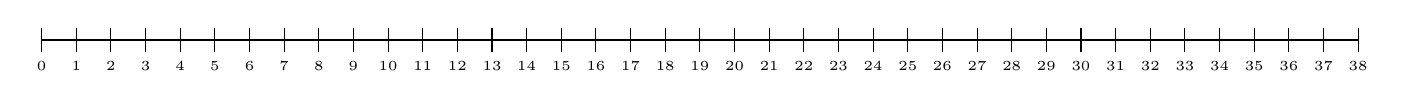
\begin{tikzpicture}[x=0.44cm, y=1cm]
    \draw[thick] (0,0) -- (38,0);
    \foreach \x in {0,...,38} {
        \draw (\x,0.15) -- (\x,-0.15);
        \node[below,font=\tiny] at (\x,-0.15) {\x};
    }
\end{tikzpicture}\\[0.05cm]
\begin{tabularx}{\textwidth}{@{} X X X @{}}
    \footnotesize Không có yếu tố đau thần kinh ($< 15\%$) / \textit{A neuropathic pain component is unlikel} & 
    \footnotesize Kết quả không rõ ràng. Có thể có đau thần kinh / \textit{Result is ambiguous, however a neuropathic pain component can be present} & 
    \footnotesize Có yếu tố đau thần kinh ($> 90\%$) / \textit{A neuropathic pain component is likely} \\
\end{tabularx}

\vspace{0.1cm}
\begin{center}
    \includegraphics[height=6.5cm,keepaspectratio]{ images/body_map_clean.png }
\end{center}



\FormFooter{ 7 }{ 19 }
\newpage

\SectionTitle{ BỘ CÂU HỎI DN4 }{ QUESTIONNAIRE DN4 }

\textbf{ Câu hỏi 1: Cơn đau hiện tại giống một hay nhiều tính chất nào dưới đây? }\\
\textit{ Question 1: Does the pain present one or more of these characteristics? }\\[0.1cm]
\noindent\CheckBox[false]{ Nóng rát/ \textit{ Burning } }\hfill\framebox[0.7cm][c]{ 1 }\par\vspace{0.08cm}
\noindent\CheckBox[false]{ Cảm giác đau lạnh/ \textit{ Painful cold } }\hfill\framebox[0.7cm][c]{ 0 }\par\vspace{0.08cm}
\noindent\CheckBox[false]{ Cảm giác điện giật/ \textit{ Electric shock } }\hfill\framebox[0.7cm][c]{ 1 }\par\vspace{0.08cm}
\vspace{0.12cm}\textbf{ Câu hỏi 2: Cơn đau cùng vị trí có liên quan đến những cảm giác dưới đây không? }\\
\textit{ Question 2: Is the pain in the same area related to one or of the following? }\\[0.1cm]
\noindent\CheckBox[false]{ Đau như kim châm/ \textit{ Pins and needles } }\hfill\framebox[0.7cm][c]{ 1 }\par\vspace{0.08cm}
\noindent\CheckBox[false]{ Đau râm ran/ \textit{ Tingling } }\hfill\framebox[0.7cm][c]{ 1 }\par\vspace{0.08cm}
\noindent\CheckBox[false]{ Tê bì/ \textit{ Numbness } }\hfill\framebox[0.7cm][c]{ 0 }\par\vspace{0.08cm}
\noindent\CheckBox[false]{ Ngứa/ \textit{ Itching } }\hfill\framebox[0.7cm][c]{ 0 }\par\vspace{0.08cm}
\vspace{0.12cm}\textbf{ Câu hỏi 3 (Khám): Đau nhiều tại vị trí được kiểm tra hay không? }\\
\textit{ Question 3 (Physician exam): Is the pain located to an area where the exam is evident? }\\[0.1cm]
\noindent\CheckBox[false]{ Mất cảm giác khi tiếp xúc (Tact hypoesthesia)/ \textit{ Tact hypoesthesia } }\hfill\framebox[0.7cm][c]{ 0 }\par\vspace{0.08cm}
\noindent\CheckBox[false]{ Mất cảm giác khi chích kim (Prick hypoesthesia)/ \textit{ Prick hypoesthesia } }\hfill\framebox[0.7cm][c]{ 0 }\par\vspace{0.08cm}
\vspace{0.12cm}\textbf{ Câu hỏi 4 (Khám): Cơn đau có tăng lên khi? }\\
\textit{ Question 4 (Physician exam): Does the pain increase by? }\\[0.1cm]
\noindent\CheckBox[false]{ Cọ xát/ \textit{ The rubbing } }\hfill\framebox[0.7cm][c]{ 1 }\par\vspace{0.08cm}

\vspace{0.3cm}
\noindent{\bfseries\large Tổng điểm/ \textit{Patient Score}:} \hfill {\Large\textbf{ N/A / 10}}



\FormFooter{ 8 }{ 19 }
\newpage

\SectionTitle{ TIÊU CHUẨN CHẨN ĐOÁN HỘI CHỨNG ĐAU VÙNG PHỨC TẠP BUDAPEST }{ BUDAPEST CRITERIA FOR COMPLEX REGIONAL PAIN SYNDROME DIAGNOSIS }

\noindent\textbf{ Hội chứng đau vùng phức tạp là đau liên tục không bị ảnh hưởng bởi với các tác nhân kích thích. Người bệnh cần có ít nhất 1 triệu chứng ở 3 trong 4 mục dưới đây: }\\
\textit{ CRPS is defined as continuing pain disproportionate to any inciting event. A patient must have at least 1 symptom in 3 of the 4 following categories: }
\vspace{0.15cm}

\textbf{ 1. Cảm giác - \textit{ Sensory }:}\par\vspace{0.05cm}
\hspace*{0.5cm}\CheckBox[false]{\textbf{ Loạn cảm đau/ \textit{ Allodynia } }}\par
\hspace*{1.0cm}\textit{\small (khi chạm nhẹ và/hoặc nhạy cảm với nhiệt độ và/hoặc áp lực cơ thể sâu và/hoặc vận động khớp)}\par
\hspace*{1.0cm}\textit{\footnotesize (to light touch and/or temperature sensation and/or deep somatic pressure and/or joint movement)}\par
\vspace{0.05cm}
\hspace*{0.5cm}\CheckBox[false]{\textbf{ Tăng cảm giác đau (châm kim)/ \textit{ Hyperalgesia (to pinprick) } }}\par
\vspace{0.05cm}
\vspace{0.12cm}
\textbf{ 2. Vận mạch - \textit{ Vasomotor }:}\par\vspace{0.05cm}
\hspace*{0.5cm}\CheckBox[false]{\textbf{ Nhiệt độ da khác nhau (>1°C) và/hoặc thay đổi màu sắc da/ \textit{ Differences in skin temperature (>1°C) and/or skin colour changes } }}\par
\vspace{0.05cm}
\hspace*{0.5cm}\CheckBox[false]{\textbf{ Khác biệt màu da ở các bên cơ thể khác nhau/ \textit{ Differences in skin colouration between different sides } }}\par
\vspace{0.05cm}
\hspace*{0.5cm}\CheckBox[false]{\textbf{ Thay đổi màu da/ \textit{ Skin colour changes } }}\par
\vspace{0.05cm}
\vspace{0.12cm}
\textbf{ 3. Bài tiết mồ hôi/Phù nề - \textit{ Sudomotor/Oedema }:}\par\vspace{0.05cm}
\hspace*{0.5cm}\CheckBox[false]{\textbf{ Hai bên cơ thể sưng nề khác nhau/ \textit{ Changes of Asymmetry in swelling } }}\par
\vspace{0.05cm}
\hspace*{0.5cm}\CheckBox[false]{\textbf{ Hai bên cơ thể toát mồ hôi khác nhau/ \textit{ Changes of Asymmetry in sweating } }}\par
\vspace{0.05cm}
\vspace{0.12cm}
\textbf{ 4. Vận động/Dinh dưỡng - \textit{ Motor/Trophic }:}\par\vspace{0.05cm}
\hspace*{0.5cm}\CheckBox[false]{\textbf{ Hạn chế vận động/ \textit{ Decreased range of movement } }}\par
\vspace{0.05cm}
\hspace*{0.5cm}\CheckBox[false]{\textbf{ Triệu chứng vận động (rùng mình, yếu ớt, rối loạn trương lực...)/ \textit{ Motor symptoms (tremor, weakness, dystonia...) } }}\par
\vspace{0.05cm}
\hspace*{0.5cm}\CheckBox[false]{\textbf{ Thay đổi về tóc, da, móng tay chân (dinh dưỡng)/ \textit{ Changes in hair, skin, nails (Trophic) } }}\par
\vspace{0.05cm}
\vspace{0.12cm}

\vspace{0.25cm}
\noindent{\bfseries Tiêu chuẩn Budapest/ \textit{Budapest criteria}:} \hspace{1cm} \CheckBox[false]{\textbf{CÓ/ \textit{YES}}} \hspace{1.5cm} \CheckBox[true]{\textbf{KHÔNG/ \textit{NO}}}


\FormFooter{ 9 }{ 19 }
\newpage

\SectionTitle{ THANG ĐÁNH GIÁ TRẦM CẢM BECK (BDI) - PHẦN 1 }{ BECK DEPRESSION INVENTORY (BDI) - PART 1 }

\noindent\textbf{ Nhóm A - Tâm trạng / Mood }\par
\NumberedOption[false]{ 0 }{ Tôi không cảm thấy buồn }{ I don't feel sad }
\NumberedOption[false]{ 1 }{ Tôi cảm thấy buồn }{ I feel sad }
\NumberedOption[false]{ 2 }{ Tôi luôn cảm thấy buồn và không thể loại bỏ nó }{ I always feel sad and I can't sort it out }
\NumberedOption[false]{ 3 }{ Tôi rất buồn và không thể chịu đựng được }{ I can't bear it }
\vspace{0.08cm}
\noindent\textbf{ Nhóm B - Bi quan / Pessimism }\par
\NumberedOption[false]{ 0 }{ Tôi không thấy bi quan về tương lai }{ I don't feel pessimistic about the future }
\NumberedOption[false]{ 1 }{ Tôi có cảm giác không tốt về tương lai }{ I have a bad feeling about future }
\NumberedOption[false]{ 2 }{ Tôi không có hy vọng gì về tương lai }{ I don't have hope }
\NumberedOption[false]{ 3 }{ Tôi không có hy vọng gì về tương lai và tình trạng này sẽ không khá hơn }{ No hope and will not be better }
\vspace{0.08cm}
\noindent\textbf{ Nhóm C - Cảm giác thất bại / Sense of failure }\par
\NumberedOption[false]{ 0 }{ Tôi không có cảm giác thất bại trong cuộc sống của mình }{ I have no sense of failure in my life }
\NumberedOption[false]{ 1 }{ Tôi có cảm giác cuộc sống của mình có nhiều thứ hơn những người khác }{ I have the feeling I have more than someone else }
\NumberedOption[false]{ 2 }{ Khi tôi nhìn lại quá khứ, tất cả những gì tôi thấy là sự thất bại }{ When I look back all I see is failure }
\NumberedOption[false]{ 3 }{ Tôi cảm thấy rằng mình đã thất bại trong chính cuộc sống của mình }{ I failed in all my personal life }
\vspace{0.08cm}
\noindent\textbf{ Nhóm D - Sự thỏa mãn / Satisfaction }\par
\NumberedOption[false]{ 0 }{ Tôi không cảm thấy thỏa mãn chút nào }{ I don't feel particularly satisfied }
\NumberedOption[false]{ 1 }{ Tôi không biết làm thế nào để thích nghi với hoàn cảnh }{ I don't know how to enjoy circumstances }
\NumberedOption[false]{ 2 }{ Tôi không thấy thỏa mãn với bất cứ điều gì }{ I don't have satisfaction with anything }
\NumberedOption[false]{ 3 }{ Tôi thấy không vui với tất cả mọi thứ }{ I am so unhappy with everything }
\vspace{0.08cm}
\noindent\textbf{ Nhóm E - Cảm giác tội lỗi / Guilt }\par
\NumberedOption[false]{ 0 }{ Tôi không cảm thấy tội lỗi }{ I don't feel guilty }
\NumberedOption[false]{ 1 }{ Tôi cảm thấy rất tệ ở mọi lúc }{ I feel so bad most of the time }
\NumberedOption[false]{ 2 }{ Tôi cảm thấy tội lỗi }{ I feel guilty }
\NumberedOption[false]{ 3 }{ Tôi thấy rất tệ và tôi nghĩ rằng tôi không xứng đáng }{ I feel bad and I am not worth it }
\vspace{0.08cm}
\noindent\textbf{ Nhóm F - Thất vọng về bản thân / Disappointed with self }\par
\NumberedOption[false]{ 0 }{ Tôi không thất vọng về bản thân mình }{ I am not disappointed with myself }
\NumberedOption[false]{ 1 }{ Tôi thất vọng về bản thân mình }{ I am disappointed by myself }
\NumberedOption[false]{ 2 }{ Tôi cảm thấy ghê tởm bản thân mình }{ I disgust myself }
\NumberedOption[false]{ 3 }{ Tôi ghét bản thân mình }{ I hate myself }
\vspace{0.08cm}
\noindent\textbf{ Nhóm G - Ý nghĩ tự làm tổn thương / Suicidal thoughts }\par
\NumberedOption[false]{ 0 }{ Tôi không nghĩ rằng sẽ làm tổn thương bản thân }{ I don't think to hurt myself }
\NumberedOption[false]{ 1 }{ Tôi nghĩ rằng cái chết sẽ giải thoát cho tôi }{ I think dying will liberate me }
\NumberedOption[false]{ 2 }{ Tôi có những kế hoạch tỉ mỉ để tự tử }{ I have precise plans to suicide }
\NumberedOption[false]{ 3 }{ Nếu có thể, tôi sẽ tự tử }{ If I can, I will kill myself }
\vspace{0.08cm}



\FormFooter{ 10 }{ 19 }
\newpage

\SectionTitle{ THANG ĐÁNH GIÁ TRẦM CẢM BECK (BDI) - PHẦN 2 }{ BECK DEPRESSION INVENTORY (BDI) - PART 2 }

\noindent\textbf{ Nhóm H - Mối quan hệ với người khác / Interest in others }\par
\NumberedOption[false]{ 0 }{ Tôi vẫn thích những người khác }{ I am still interested in other people }
\NumberedOption[false]{ 1 }{ Hiện nay tôi ít hứng thú với những người khác }{ Now, I am less interested in others }
\NumberedOption[false]{ 2 }{ Tôi mất hết cảm giác với những người khác và không cảm thấy gì về họ cả }{ Lost all interest in others }
\NumberedOption[false]{ 3 }{ Tôi mất hết cảm giác với những người khác và không quan tâm về nó }{ Lost interest and don't care }
\vspace{0.08cm}
\noindent\textbf{ Nhóm I - Khả năng ra quyết định / Decision making }\par
\NumberedOption[false]{ 0 }{ Tôi vẫn có thể đưa ra quyết định }{ I am still capable to take decisions }
\NumberedOption[false]{ 1 }{ Tôi đang cố tránh đưa ra quyết định }{ Trying to avoid taking decisions }
\NumberedOption[false]{ 2 }{ Thật khó để đưa ra quyết định }{ It is hard to take decisions }
\NumberedOption[false]{ 3 }{ Tôi không thể đưa ra quyết định }{ Uncapable to take decisions }
\vspace{0.08cm}
\noindent\textbf{ Nhóm J - Hình ảnh bản thân / Body image }\par
\NumberedOption[false]{ 0 }{ Tôi không cảm thấy mình xấu xí }{ I don't have the feeling that I look ugly }
\NumberedOption[false]{ 1 }{ Tôi sợ già }{ I am afraid to look old }
\NumberedOption[false]{ 2 }{ Tôi cảm thấy có gì đó về ngoại hình khiến tôi trở nên thật xấu xí }{ Something makes me look ugly }
\NumberedOption[false]{ 3 }{ Tôi cảm thấy mình trông thật tệ }{ I feel that I look bad }
\vspace{0.08cm}
\noindent\textbf{ Nhóm K - Khả năng làm việc / Work ability }\par
\NumberedOption[false]{ 0 }{ Tôi làm việc dễ dàng như trước }{ I work as easy as before }
\NumberedOption[false]{ 1 }{ Tôi cần một chút nỗ lực }{ I need to do some effort }
\NumberedOption[false]{ 2 }{ Tôi cần rất nhiều nỗ lực mà không làm được gì }{ Need a lot of effort to do anything }
\NumberedOption[false]{ 3 }{ Tôi không thể làm gì kể cả việc nhỏ nhất }{ Uncapable to do the smallest job }
\vspace{0.08cm}
\noindent\textbf{ Nhóm L - Mệt mỏi / Fatigue }\par
\NumberedOption[false]{ 0 }{ Tôi không mệt mỏi như mọi khi }{ I am not so tired like usual }
\NumberedOption[false]{ 1 }{ Tôi thấy mệt mỏi rất dễ dàng }{ I get tired easily }
\NumberedOption[false]{ 2 }{ Không làm gì cũng khiến tôi mệt mỏi }{ Doing anything makes me tired }
\NumberedOption[false]{ 3 }{ Tôi không thể làm bất cứ công việc gì }{ Not able to do any work }
\vspace{0.08cm}
\noindent\textbf{ Nhóm M - Sự ngon miệng / Appetite }\par
\NumberedOption[false]{ 0 }{ Tôi ăn ngon miệng }{ I have a good appetite }
\NumberedOption[false]{ 1 }{ Tôi không thấy ngon miệng như mọi khi }{ I don't have good appetite like usual }
\NumberedOption[false]{ 2 }{ Bữa ăn của tôi tệ hơn trước rất nhiều }{ My appetite is much worse }
\NumberedOption[false]{ 3 }{ Tôi không cảm thấy ngon miệng chút nào }{ I lost my appetite }
\vspace{0.08cm}

\vspace{0.2cm}
\begin{flushright}
    \small\bfseries KẾT QUẢ/ RESULTS:\\[0.05cm]
    0 đến 3: không có trầm cảm/ \textit{0 to 3: no depression}\\
    4 đến 7: trầm cảm nhẹ/ \textit{4 to 7: mild depression}\\
    8 đến 15: trầm cảm ở mức độ vừa/ \textit{8 to 15: moderate depression intensity}\\
    Từ 16 trở lên: trầm cảm nặng/ \textit{16 and above: severe depression}
\end{flushright}


\FormFooter{ 11 }{ 19 }
\newpage


\begin{center}
    {\bfseries\Large SƠ ĐỒ CẢM GIÁC TOÀN THÂN (MẶT TRƯỚC \& MẶT SAU)}\\[0.05cm]
    {\bfseries\large FULL BODY SENSORY PROFILE (ANTERIOR \& POSTERIOR VIEW)}
\end{center}
\vspace{0.15cm}

\textbf{Bác sỹ điều trị/ \textit{Physician}:} \dotfill\\[0.12cm]
\textbf{Ngày/ \textit{Date}:} \dotfill ~~~~~ \textbf{Giờ/ \textit{Time}:} \dotfill
\vspace{0.15cm}

\begin{center}
    \includegraphics[height=17.5cm,keepaspectratio]{ images/full_body_sensory_anterior_posterior.png }
\end{center}



\FormFooter{ 12 }{ 19 }
\newpage


\begin{center}
    {\bfseries\Large SƠ ĐỒ CẢM GIÁC TOÀN THÂN (TƯ THẾ NGHIÊNG)}\\[0.05cm]
    {\bfseries\large FULL BODY SENSORY PROFILE (LATERAL VIEW)}
\end{center}
\vspace{0.15cm}

\textbf{Bác sỹ điều trị/ \textit{Physician}:} \dotfill\\[0.12cm]
\textbf{Ngày/ \textit{Date}:} \dotfill ~~~~~ \textbf{Giờ/ \textit{Time}:} \dotfill
\vspace{0.15cm}

\begin{center}
    \includegraphics[height=17.5cm,keepaspectratio]{ images/full_body_sensory_lateral.png }
\end{center}



\FormFooter{ 13 }{ 19 }
\newpage


\begin{center}
    {\bfseries\Large SƠ ĐỒ KHÁM CẢM GIÁC CỤC BỘ (MẶT, BÀN TAY, VÙNG KÍN)}\\[0.05cm]
    {\bfseries\large FOCAL SENSORY EXAMINATION MAPS (FACE, HANDS, PERINEAL)}
\end{center}
\vspace{0.15cm}

\textbf{Bác sỹ điều trị/ \textit{Physician}:} \dotfill\\[0.12cm]
\textbf{Ngày/ \textit{Date}:} \dotfill ~~~~~ \textbf{Giờ/ \textit{Time}:} \dotfill
\vspace{0.15cm}

\begin{center}
    \includegraphics[height=17.5cm,keepaspectratio]{ images/physician_focal_clean.png }
\end{center}



\FormFooter{ 14 }{ 19 }
\newpage

\SectionTitle{ THÔNG TIN QUAN SÁT }{ OBSERVATION }

\SectionTitle{ Ghi chú quan sát lâm sàng: }{ Physician Clinical Observation: }

\noindent\dotfill\\[0.35cm]
\noindent\dotfill\\[0.35cm]
\noindent\dotfill\\[0.35cm]

\SubSectionTitle{ BẢNG ĐIỀU TRỊ }{ TREATMENTS TABLE }

\noindent
\begin{tabularx}{\textwidth}{|X|c|c|X|X|}
    \hline
    \rowcolor{gray!15}
    \textbf{\small Điều trị} & 
    \textbf{\small Ngày} & 
    \textbf{\small Thời gian} & 
    \textbf{\small Khả năng thích ứng của NB} & 
    \textbf{\small Tác dụng} \\
    \rowcolor{gray!15}
    \textit{\footnotesize Treatments} & 
    \textit{\footnotesize Date} & 
    \textit{\footnotesize Duration} & 
    \textit{\footnotesize Tolerability} & 
    \textit{\footnotesize Effect} \\
    \hline
        NSAID (Celecoxib) 200mg & 
        30/09/2026 & 
        2 tuần & 
        1 viên/ngày sau ăn (uống sau ăn no) & 
        Kháng viêm, giảm triệu chứng đau \\ \hline
        Vật lý trị liệu phục hồi chức năng (Viêm quanh khớp vai / rách gân chóp xoay) & 
        30/09/2026 & 
        3-4 tuần (3 buổi/tuần) & 
        Tập vận động nhẹ nhàng theo hướng dẫn kỹ thuật viên & 
        Chống dính khớp, phục hồi biên độ cử động \\ \hline
\end{tabularx}

\FormFooter{ 15 }{ 19 }
\newpage

\SectionTitle{ TỔNG HỢP KẾT QUẢ }{ SYNTHESIS }

\textbf{ Chẩn đoán mức độ tổn thương dựa trên đo lường/ \textit{ Topographic diagnostic of the lesion level }: } \underline{~Viêm quanh khớp vai / rách gân chóp xoay~}\\[0.12cm]
\textbf{ Chẩn đoán căn nguyên/ \textit{ Diagnostic Etiology }: } \underline{~Thoái hóa gân kết hợp vi chấn thương do vận động lặp đi lặp lại~}\\[0.12cm]
\textbf{ Đau khó chịu nhất hoặc vị trí đau xác định là/ \textit{ The most annoying pain or target pain }: } \underline{~Khớp vai tổn thương, buốt nhức nhiều về đêm~}\\[0.12cm]

\SubSectionTitle{ YẾU TỐ CĂN NGUYÊN }{ ETIOLOGICAL FACTOR }

\textbf{ Nhiễm trùng/ \textit{ Infectious }: } \underline{~N/A~}\\[0.12cm]
\textbf{ Chấn thương/ \textit{ Traumatic }: } \underline{~Tiền sử chấn thương ngã trước đây~}\\[0.12cm]
\textbf{ Mạch máu/ \textit{ Vascular }: } \underline{~N/A~}\\[0.12cm]
\textbf{ Chuyển hóa/ \textit{ Metabolic }: } \underline{~N/A~}\\[0.12cm]
\textbf{ Viêm nhiễm/ \textit{ Inflammatory }: } \underline{~Viêm vô khuẩn bao hoạt dịch và gân cơ~}\\[0.12cm]
\textbf{ Nhiễm độc/ \textit{ Toxic }: } \underline{~N/A~}\\[0.12cm]
\textbf{ Khác/ \textit{ Other }: } \underline{~N/A~}\\[0.12cm]


\FormFooter{ 16 }{ 19 }
\newpage

\SectionTitle{ ĐIỀU TRỊ CÓ XÂM LẤN }{ INVASIVE TREATMENT }

\SubSectionTitle{ Nếu thủ thuật có xâm lấn được đề xuất }{ If an invasive procedure is proposed }

\textbf{ Loại thủ thuật/ \textit{ Type of procedure }: } \underline{~N/A~}\\[0.12cm]
\textbf{ Mức độ/ \textit{ Level }: } \underline{~N/A~} ~~~~~ \textbf{ Loại block/ \textit{ Type of block }: } \underline{~N/A~} ~~~~~ \textbf{ Side/ \textit{ Side }: } \underline{~N/A~}\\[0.12cm]
\textbf{ Mã ICD10/ \textit{ ICD10 }: } \underline{~N/A~} ~~~~~ \textbf{ Mã CPT/ \textit{ CPT }: } \underline{~N/A~}\\[0.12cm]
\textbf{ Ngày/ \textit{ Date }: } \underline{~N/A~} ~~~~~ \textbf{ Giờ/ \textit{ Time }: } \underline{~N/A~}\\[0.12cm]

\begin{tabularx}{\textwidth}{@{} X @{}}
    \CheckBox[false]{ Thông tin về lợi ích và nguy cơ đã được giải thích cho người bệnh/ \textit{ Oral Information Benefits risks } }   \\[0.12cm]
    \CheckBox[false]{ Hướng dẫn người bệnh về thủ tục nhập viện/ \textit{ Patient instructions for the admission } }   \\[0.12cm]
    \CheckBox[false]{ Hướng dẫn người bệnh về giá/ \textit{ Information concerning price } }   \\[0.12cm]
    \CheckBox[false]{ Thông tin đã được ghi chép/ \textit{ Written information } }   \\[0.12cm]
\end{tabularx}
\textbf{ PHIẾU CAM KẾT ĐƯỢC KÝ VÀO NGÀY LÀM THỦ THUẬT/ \textit{ CONSENT WILL BE SIGN THE DAY OF THE PROCEDURE }: } \underline{~N/A~}\\[0.12cm]

\SectionTitle{ Báo cáo thủ thuật: }{ Procedure Report: }

\noindent\dotfill\\[0.35cm]
\noindent\dotfill\\[0.35cm]
\noindent\dotfill\\[0.35cm]
\noindent\dotfill\\[0.35cm]


\FormFooter{ 17 }{ 19 }
\newpage

\SectionTitle{ CHẨN ĐOÁN ĐỊNH HƯỚNG }{ DIAGNOSTIC ORIENTATION }

\SubSectionTitle{ - Đau TK ngoại biên }{ Peripheral neuropathic pain }

\begin{tabularx}{\textwidth}{@{} X X X @{}}
    \CheckBox[false]{ TK dưới da/ \textit{ Superficial shootskin } }  &     \CheckBox[false]{ Trục TK/ \textit{ Troncular } }  &     \CheckBox[false]{ Rễ TK/ \textit{ Radicular } }   \\[0.12cm]
\end{tabularx}
\SubSectionTitle{ - Đau TK trung ương }{ Central Neuropathic pain }

\begin{tabularx}{\textwidth}{@{} X X @{}}
    \CheckBox[false]{ Tủy sống/ \textit{ Medullar } }  &     \CheckBox[false]{ Cạnh tủy sống/ \textit{ Supra-medullar } }   \\[0.12cm]
\end{tabularx}
\SubSectionTitle{ TỔNG HỢP: ĐÁNH GIÁ YÊU CẦU CỦA NGƯỜI BỆNH }{ SYNTHESIS: EVALUATION OF THE PATIENT REQUEST }

\textbf{ - Ưu tiên của người bệnh là gì?/ \textit{ What is the patient priority? }: } \underline{~Hết đau nhức ban đêm để có giấc ngủ ngon và cử động cánh tay linh hoạt~}\\[0.12cm]
\textbf{ - Mức độ cải thiện chung mà người bệnh có thể chấp nhận? Tỷ lệ cải thiện/ \textit{ What level of overall improvement is he ready to accept? Percentage of amelioration }: } \underline{~N/A~}\\[0.12cm]
\textbf{ - Thái độ của NB đối với các phương pháp điều trị đặc biệt? (Thuốc chống trầm cảm hoặc suy nhược)/ \textit{ What is his attitude regarding a specific treatment? (Antiepileptic or antidepressant) }: } \underline{~N/A~}\\[0.12cm]
\textbf{ Đề xuất kế hoạch/ \textit{ Strategy proposed }: } \underline{~Phối hợp thuốc giảm đau chống viêm non-steroid + Thuốc giãn cơ + Tập VLTL phục hồi chức năng~}\\[0.12cm]
\textbf{ Lợi ích/ \textit{ Benefits }: } \underline{~Cắt cơn đau viêm cấp, phòng ngừa cứng dính khớp~} ~~~~~ \textbf{ Tỷ lệ thành công/ \textit{ Success rate }: } \underline{~85\%~}\\[0.12cm]
\textbf{ Nguy cơ/ \textit{ Risks }: } \underline{~N/A~}\\[0.12cm]
\textbf{ Người bệnh đồng ý/ \textit{ Patient acceptance }: } \underline{~Có / Yes~}\\[0.12cm]


\FormFooter{ 18 }{ 19 }
\newpage

\SectionTitle{ THEO DÕI \& LỊCH TRÌNH TÁI KHÁM }{ FOLLOW UP \& NEXT VISITS }

\FollowUpBlock
\FollowUpBlock
\FollowUpBlock
\FollowUpBlock
\FollowUpBlock
\FollowUpBlock
\FollowUpBlock


\FormFooter{ 19 }{ 19 }

\end{document}